63. \begin{figure}[ht!]
\center{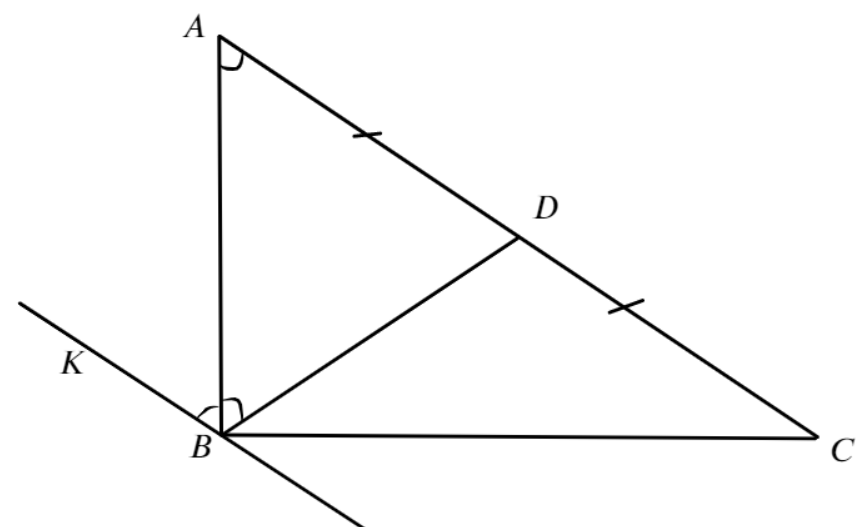
\includegraphics[scale=0.35]{g63.png}}
\end{figure}\\
Углы $KBA$ и $BAD$ являются накрест лежащими при параллельных прямых $KB$ и $AC,$ значит $\angle ABD=\angle KBA=\angle BAD.$ Поэтому треугольник $ABD$ является равнобедренным и $AD=BD,$ а значит равнобедренным является и треугольник $BDC$ (так как $AD=DC,\ BD$ --- медиана). Обозначим их углы при основании $\angle BAD=\angle ABD=x,\ \angle BCD=\angle CBD=y,$ тогда из треугольника $ABC$ имеем $2x+2y=180^\circ,\ x+y=90^\circ=\angle ABC,$ ч.т.д.\\
